% Capítulo 8: merge sort, dividindo até sobrar um elemento e intercalando de volta.
% Gerado a partir das posições calculadas (8 casas, grupos de 8, 4, 2 e 1).
\documentclass[border=4pt]{standalone}
\usepackage[utf8]{inputenc}
\usepackage[T1]{fontenc}
% Estilo comum das figuras de vetores (capítulo 8).
\usepackage{tikz}
\usetikzlibrary{arrows.meta, positioning, calc, decorations.pathreplacing}
\definecolor{navy}{RGB}{23,45,80}
\definecolor{laranja}{RGB}{250,110,29}
\definecolor{cinzalogo}{RGB}{107,114,126}
\definecolor{azul}{RGB}{205,222,247}
\tikzset{
  casa/.style={draw=navy, line width=0.9pt, minimum width=8mm, minimum height=7mm,
               inner sep=0pt, font=\sffamily\small},
  pronta/.style={casa, fill=azul},
  parte/.style={casa, fill=laranja!12},
  marcada/.style={casa, fill=laranja!45, draw=laranja},
  fora/.style={casa, draw=cinzalogo!60, dashed, fill=white, text=cinzalogo!60},
  indice/.style={font=\sffamily\scriptsize, text=cinzalogo},
  explica/.style={font=\sffamily\small, text=navy, anchor=east},
  legenda/.style={font=\sffamily\scriptsize, text=cinzalogo},
  rotulo/.style={font=\sffamily\small\bfseries, text=navy},
  seta/.style={-{Stealth[length=2.2mm]}, navy, line width=0.9pt},
  chave/.style={decorate, decoration={brace, amplitude=4pt, mirror}, navy, line width=0.8pt},
}
% \vetor{nome}{x}{y}{valor/estilo, valor/estilo, ...}: casas lado a lado, chamadas nome0, nome1...
\newcommand{\vetor}[4]{%
  \foreach \valor/\estilo [count=\i from 0] in {#4} {
    \node[\estilo] (#1\i) at ($(#2, #3) + (\i*0.8, 0)$) {\valor};
  }
}

\begin{document}
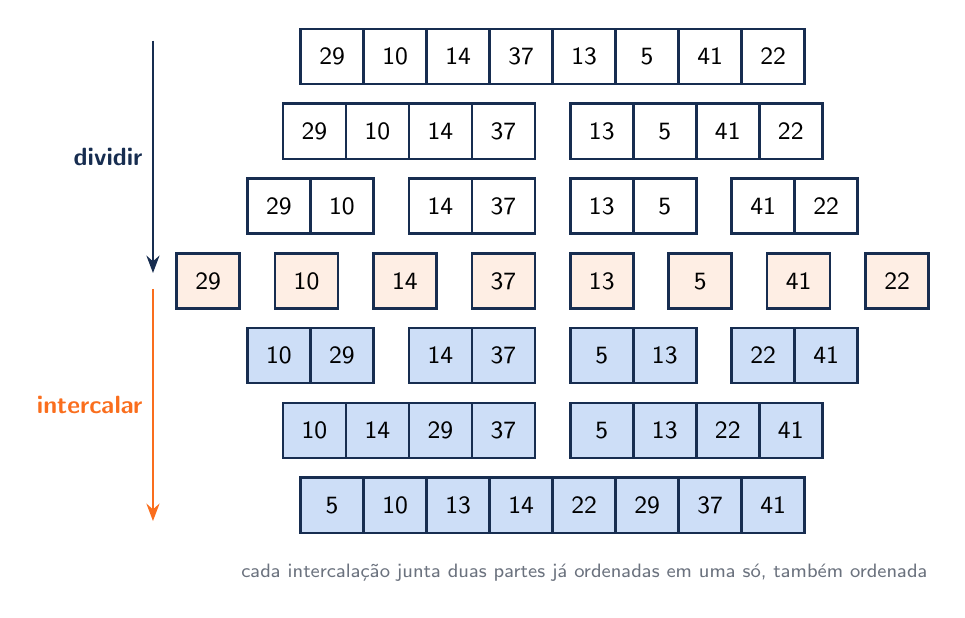
\begin{tikzpicture}
  \node[casa] at (1.575, 0.00) {29};
  \node[casa] at (2.375, 0.00) {10};
  \node[casa] at (3.175, 0.00) {14};
  \node[casa] at (3.975, 0.00) {37};
  \node[casa] at (4.775, 0.00) {13};
  \node[casa] at (5.575, 0.00) {5};
  \node[casa] at (6.375, 0.00) {41};
  \node[casa] at (7.175, 0.00) {22};
  \node[casa] at (1.350, -0.95) {29};
  \node[casa] at (2.150, -0.95) {10};
  \node[casa] at (2.950, -0.95) {14};
  \node[casa] at (3.750, -0.95) {37};
  \node[casa] at (5.000, -0.95) {13};
  \node[casa] at (5.800, -0.95) {5};
  \node[casa] at (6.600, -0.95) {41};
  \node[casa] at (7.400, -0.95) {22};
  \node[casa] at (0.900, -1.90) {29};
  \node[casa] at (1.700, -1.90) {10};
  \node[casa] at (2.950, -1.90) {14};
  \node[casa] at (3.750, -1.90) {37};
  \node[casa] at (5.000, -1.90) {13};
  \node[casa] at (5.800, -1.90) {5};
  \node[casa] at (7.050, -1.90) {41};
  \node[casa] at (7.850, -1.90) {22};
  \node[parte] at (0.000, -2.85) {29};
  \node[parte] at (1.250, -2.85) {10};
  \node[parte] at (2.500, -2.85) {14};
  \node[parte] at (3.750, -2.85) {37};
  \node[parte] at (5.000, -2.85) {13};
  \node[parte] at (6.250, -2.85) {5};
  \node[parte] at (7.500, -2.85) {41};
  \node[parte] at (8.750, -2.85) {22};
  \node[pronta] at (0.900, -3.80) {10};
  \node[pronta] at (1.700, -3.80) {29};
  \node[pronta] at (2.950, -3.80) {14};
  \node[pronta] at (3.750, -3.80) {37};
  \node[pronta] at (5.000, -3.80) {5};
  \node[pronta] at (5.800, -3.80) {13};
  \node[pronta] at (7.050, -3.80) {22};
  \node[pronta] at (7.850, -3.80) {41};
  \node[pronta] at (1.350, -4.75) {10};
  \node[pronta] at (2.150, -4.75) {14};
  \node[pronta] at (2.950, -4.75) {29};
  \node[pronta] at (3.750, -4.75) {37};
  \node[pronta] at (5.000, -4.75) {5};
  \node[pronta] at (5.800, -4.75) {13};
  \node[pronta] at (6.600, -4.75) {22};
  \node[pronta] at (7.400, -4.75) {41};
  \node[pronta] at (1.575, -5.70) {5};
  \node[pronta] at (2.375, -5.70) {10};
  \node[pronta] at (3.175, -5.70) {13};
  \node[pronta] at (3.975, -5.70) {14};
  \node[pronta] at (4.775, -5.70) {22};
  \node[pronta] at (5.575, -5.70) {29};
  \node[pronta] at (6.375, -5.70) {37};
  \node[pronta] at (7.175, -5.70) {41};
  \draw[seta] (-0.7, 0.20) -- (-0.7, -2.75) node[midway, rotulo, left] {dividir};
  \draw[seta, laranja] (-0.7, -2.95) -- (-0.7, -5.90) node[midway, rotulo, left, text=laranja] {intercalar};
  \node[legenda] at (4.78, -6.55) {cada intercalação junta duas partes já ordenadas em uma só, também ordenada};
\end{tikzpicture}
\end{document}
